\documentclass[
    10pt,
    a4paper,
    % twocolumn,
    % twoside=semi
    ]{article}

\usepackage{aas_macros}
\usepackage{natbib}
\bibpunct{(}{)}{;}{a}{}{,}

\usepackage{geometry}
\geometry{
    paper=letterpaper, % Change to letterpaper for US letter
    top=2cm,           % Top margin
    bottom=2cm,        % Bottom margin
    left=2cm,          % Left margin
    right=2cm,         % Right margin
    % showframe,
    }

\usepackage{printlen}
% \uselengthunit{in}\printlength{\textwidth}

\usepackage{graphicx}
\graphicspath{{figures}}
\usepackage{booktabs}

\usepackage[super]{nth}
\usepackage{siunitx}
\DeclareSIUnit{\parsec}{pc}
\DeclareSIUnit{\arcsec}{asec}
\DeclareSIUnit{\erg}{erg}
\DeclareSIUnit{\arcmin}{arcmin}
\DeclareSIUnit{\arcsec}{arcsec}
\DeclareSIUnit{\mas}{mas}
\sisetup{
    range-phrase=\text{--},
    range-units=single
    }

% \usepackage{tex4ebook}
\usepackage{tikz}
\usetikzlibrary{calc}

\usepackage{amsmath,amssymb}
\usepackage{mathtools}
\usepackage{commath}
\usepackage{upgreek}
\usepackage{enumerate}

\usepackage{hyperref}
\hypersetup{
    pdffitwindow=true,
    pdfstartview={FitH},
    pdftitle={This is a report},
    pdfauthor={Tomas Cassanelli},
    pdfcreator={Tomas Cassanelli},
    pdfproducer={Tomas Cassanelli},
    pdfnewwindow=true,
    colorlinks=true,
    linkcolor=red,
    citecolor=magenta,
    urlcolor=blue
    }
    

\usepackage{lipsum}  % remove this line

\begin{document}

\title{Report template}
\author{Tom\'{a}s Cassanelli et al.}
\date{\today}

\maketitle

\section{Introduction}
\label{sec:introduction}

This is a small report template. The idea of this sort of report is to be 1--3 pages long describing a problem and potential solution.

\section{Tables}
To make nice tables we suggest the package \texttt{booktabs}, as shown in Table \ref{tab:my_table}. This lets you add bar lines and make the tables more compact. Since it is a matter of taste feel free to look for your preferred one

\begin{table}[t]
    \centering
    \begin{tabular}{ccc}
        \toprule
        \textbf{A} & \textbf{B} & \textbf{C} \\ \midrule
        1 & 2 & 3 \\
        1 & 2 & 3 \\
        1 & 2 & 3 \\
        1 & 2 & 3 \\
        1 & 2 & 3 \\
        \bottomrule
    \end{tabular}
    \caption{Adding a caption}
    \label{tab:my_table}
\end{table}

\section{Making your own figures}

To make figures using Python it is recommended to use the style file \texttt{plot\_scripts/paper\_sty.mplstyle}, so your figures will have the same text size and shape as this document (see the \texttt{plot\_scripts/dummy.py} example).
To check the maximum length (or width) that your figures may have use the following \LaTeX~package \texttt{printlength} for example the current width is: \uselengthunit{in}\printlength{\textwidth}. There is an example of a Python script and its figure in Fig.~\ref{fig:dummy}.
 
\begin{figure}
    \centering
    \includegraphics{dummy.pdf}
    \caption{This is a figure made with the script in \texttt{plot\_scripts/dummy.py}, the figure has the same font format as this caption and text in the document. Notice that $x$-axis and $y$-axis have been written in math mode within the figure labels.}
    \label{fig:dummy}
\end{figure}

\subsection{Ti\textit{k}Z figures}
Ti\textit{k}Z  (PGF plots) is a powerful tool to create in-line-figures in \LaTeX. Unfortunately the learning curve is very steep, but it is definitely worth learning it! There are several online examples that you can browse and edit. Making your own figures will always have an extra value in your report and it is highly appreciated. Source to learn how to make figures are:
\begin{itemize}
    \item The Ti\textit{k}Z package manual, it is long and sometimes misleading but if you want to master Ti\textit{k}Z is the right place to start!
    \item \url{https://www.ctan.org/pkg/pgf}
    \item Several cool examples: \url{http://www.texample.net/}.
    \item Brief introduction: \url{https://www.sharelatex.com/learn/TikZ_package}
\end{itemize}

With some command lines you can make something like in Fig.~\ref{fig:my_tikz_fig}.

\begin{figure}[h]
    \centering
    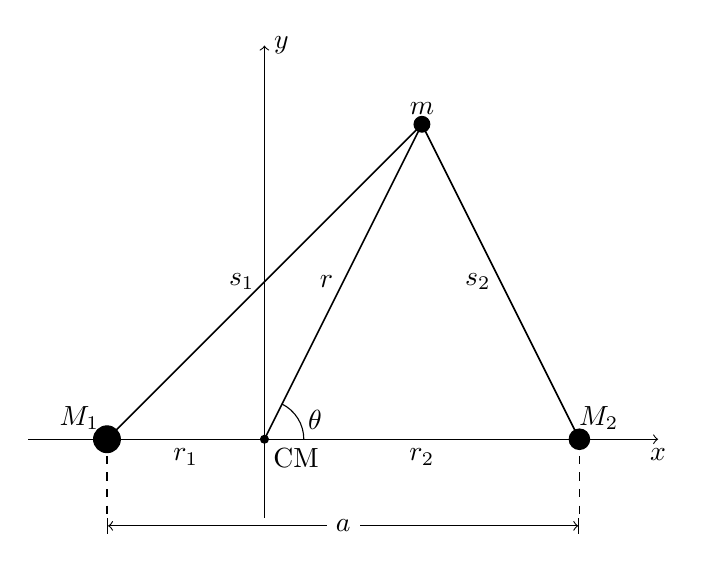
\begin{tikzpicture}

        \def\linethick{0.6pt}

        \coordinate (M1) at (-2, 0);
        \coordinate (m) at (2, 4);
        \coordinate (M2) at (4, 0);

        \draw[->] (-3, 0) -- (5, 0) node[left, below] {$x$};
        \draw[->] (0, -1) -- (0, 5) node[right] {$y$};

        \draw[line width=\linethick] (0, 0) -- node[midway,left] {$r$} (m) node[above] {$m$};
        \draw[line width=\linethick] (M1) node[above, xshift=-10] {$M_1$} -- node[midway,left] {$s_1$} (m);
        \draw[line width=\linethick] (M2) node[above, xshift=7] {$M_2$} -- node[midway,left] {$s_2$} (m);

        \path (M1) -- node[midway, below] {$r_1$} (0, 0);
        \path (0, 0) -- node[midway, below] {$r_2$} (M2);

        % Dashed lines
        \draw[dashed] (M1) -- ++ (0, -1);
        \draw[dashed] (M2) -- ++ (0, -1);

        \draw[|<->|] ($(M1) + (0, -1.1)$) -- node[midway,fill=white] {$a$} ($(M2) + (0, -1.1)$);

        \node[below] at (0.4, 0) {CM};

        \draw ([shift={(0, 0)}]64:0.5) arc[radius=0.5, start angle=64, end angle=0] node[above, xshift=4] {$\theta$};

        % balck circles
        \filldraw[black] (m) circle(0.1);
        \filldraw[black] (M1) circle(0.17);
        \filldraw[black] (M2) circle(0.13);
        \filldraw[black] (0, 0) circle(0.05);

    \end{tikzpicture}
    \caption{Nice diagram using Ti\textit{k}Z. Notice that the typesetting of variables is the same as the one used in \LaTeX. Variables $\theta$, $M_1$, $M_2$, have the same font and text style.}
    \label{fig:my_tikz_fig}
\end{figure}

To add a citation we use the \textit{natbib} package, which is the standard way of citation in natural sciences, a citation example would be like this \citep{2022A&A...663A.106C}.
\noindent The in-line citations are:
\begin{itemize}
    \item \citep{2022A&A...663A.106C}
    \item \citet{2022A&A...663A.106C}
    \item \citep[see][]{2022A&A...663A.106C}
\end{itemize}

\section{Units and describing quantities}

I recommend using the \texttt{siunitx} package, to properly write units and numbers in \LaTeX, makes life so much easier, an example of this would be:
\begin{equation}
    I_\nu\del{\nu,\widehat{\mathbf{n}}, \mathbf{r}, t}\dif\nu\dif\Omega \, \unit{\watt\per\m\squared}.
    \label{eq:specific_intensity}
\end{equation}
In Eq.~\eqref{eq:specific_intensity} we have added the units in math mode, they also work on text mode, e.g., \unit{\watt\per\m\squared}. 

For more about the units see the online documentation \url{https://ctan.org/pkg/siunitx}.

\section{Lipsum}
\lipsum[2-4]

\bibliographystyle{bibstyle_aa.bst}
\bibliography{report_template}

\end{document}
